This chapter introduces the notion of language drift and reviews work investigating this phenomenon. More specifically, language drift in context of neural agents generating natural language is considered. Natural language used by humans is also subject to various changes like lexical semantic changes \parencite{blank1999new}, subjectification of certain propositions \parencite{traugott1989rise},  and general adaptation of language to usage contexts \parencite{five2009language}. Yet it is left to future work to zoom in on the relation between language change and language drift in multi-agent communication. 

Literature on reinforcement learning often distinguishes between \textit{structural} (also sometimes called \textit{syntactic}), \textit{semantic} and \textit{pragmatic} drift \parencite{lazaridou2020multi}.
First, prior work addressing language drift is reviewed in Section \ref{ld_mitigation}. Second, metrics aiming to capture these different kinds of drift which are also used in presented experiments are reviewed in Section \ref{ld_metrics}. Then, novel aspects in investigating language drift tested in this thesis are described. Finally, specific hypotheses regarding expected language drift in the presently conducted experiments are presented in Section \ref{hypos}. 

\section{Mitigating Language Drift}
\label{ld_mitigation}
The phenomenon of \textit{language drift} was first detected by \cite{lewis2017deal} who trained artificial agents to cooperate on a negotation task in natural language, given a corpus of human dialogues. They showed that the negotiation skills were significantly improved by optimizing the pretrained sequence-to-sequence agents with a preformance-based reward via REINFORCE. However, this came at a cost of divergence from human language---i.e., the human intelligibility of the communication produced by the agents drastically decreased. This phenomenon is called language drift. To combat that, they switched between reinforcment learning and supervised learning. However, no precise quantification of the drift was presented. 

Building upon this work, \cite{lee2019countering} counteracted drift by imposing a supervised learning constraint on the produced language. Specifically, their agents played a multi-modal translation game wherein the first agent was tasked with the translation of a sequence from French to English and the second---from English to German. Both agents were pretrained on the translation task before the communication game. The pivot language English was used in order to investigate language drift as the agents were trained on French-German translation with REINFORCE. They compared the mitigation of language drift through a language modeling constraint (i.e., incorporating the maximization of the likelihood of the English sentence under a pretrained LM into the reward) to grounding (i.e., maximizing the likelihood of an image corresponding to the English sentence under a pretrained image retrieval model). The first constraint mainly preserved the \textit{surface structure} of the learned language, while the second enforced correct semantics, i.e., the use of correct words with respect to visual inputs. The first approach is also similar to the supervised training employed by \cite{lewis2017deal}, and the second is related to the listener component of the noisy channel model by \cite{lazaridou2020multi} (see Section \ref{mac}).
\cite{lee2019countering} first estimated language drift within the evaluation of the overall translation quality by reporting BLEU scores (see Section \ref{image_cap_metrics}). They observed a drop in French-English translation scores in the vanilla model without constraints when the scores for the French-German performance increased. The highest scores were achieved with the model containing both constraints, both on French-Eglish and the French-German translation. LM regularization has shown better improvement of the English scores, though this was partly due to the preference of the BLEU score for the surface form which was better regulated by an LM. Yet combining the LM and the image retrieval model yielded the best results, indicating that the drift may also occur at semantic level, which was mitigated by grounding. Second, they looked at by part-of-speech recall at inference time, finding that the vanilla model had difficulties with function words as well as produced a flatter token distribution, compared to the combined regularization model. Further, the vanilla model was more prone to repeating words. To sum up, their results suggest that both syntactic and semantic drift take place when optimizing agents with external task rewards. However, they captured the drift by task-specific metrics (i.e., translation BLEU scores) which might make it difficult to extend their diagnostics to other experiments. Nonetheless, their work inspired some evaluation approaches used in this thesis (see below).

A different approach to mitigating language drift, rather focusing on stabilizing the language by creating community pressures on the agents, was taken by \cite{lu2020countering}. They tested the so-called \textit{seeded iterated learning} (SIL) approach whereby they periodically finetuned the pretrained speaker agent to imitate the behavior of a teacher agent fine-tuned on the task. It was motivated by iterated learning models which are prominent in research on emergence and evolution of language structure \parencite{kirby2014iterated}. More precisely, the teacher agent was initially a duplicate of the learning speaker agent which essentially provided the \textit{seed} for the supervision iterations. The imitation sequences consisted of supervised training on data sampled from the fine-tuned teacher agent. They tested this approach on a reference game and the translation game from \cite{lee2019countering}. The success of countering the drift in the reference game was measured via the ``Sender Language Score'' and the ``Task Scores'' (p. 5). The former compared the generated and ground-truth captions by-token. The latter was the referential accuracy. % The SIL model was shown to outperform several baselines.
For the latter task the drift was measured via BLEU scores, negative log likelihood of the messages (NLL, for capturing structural drift) and ranking scores under a pretrained image ranker (for capturing semantic drift). The SIL model was shown to be more robust against BLEU, ranking and NLL decreases than baselines.
%--  evolutionary / community / stabilisation via listener variation / against coadaptation.

Since this thesis replicates and extends the work by \cite{lazaridou2020multi} described in Section \ref{multi_agent_arch}, their approach to capturing language drift is discussed in more detail.
Different from previous work which focused on the speaker architecture only, in order to investigate language drift, they conducted a set of evaluations of the sender agents by varying the \emph{receiver} agent. They evaluated the different speakers trained simulataneously with a listener against the same \textit{joint} listener, a \textit{fixed} pretrained listener and a human, using an easy and difficult test set consisting of 1000 image pairs each. Furthermore, they varied the source of the samples for the reranker models (see Section \ref{multi_agent_arch}): they were either the ground truth captions or samples from an image captioner pretrained on single image captioning only. As a baseline, they had human speakers pick the most discriminative caption among the ground truth options for a human listener and achieved an acuracy of 0.97. By contrast, the reranker model operating on the ground truth captions trained against a joint listener only achieved an accuracy of 0.92 with human listeners, indicating that the capacity of the listener and reranker modules were somewhat below human performance. They found that the noisy channel speaker performed best with humans when trained with a joint listener, while the PoE model performed best with humans when reranking ground truth captions. Investigating the reasons for language drift, they found that the \emph{speaker-listener co-adaptation} (i.e., agents' forming of conventions as the are jointly trained) had the least effect on the noisy channel speaker (human performance was 0.86 vs 0.87 for joint versus fixed speaker training), and had most significant effect on the reward finetuning speaker with KL regularization (human performance was 0.69 vs. 0.0.75). The PoE speaker was also the most robust against structural and semantic drifts. Finally, they found that unfreezing the visual model weights incresed the gap between the performance of the joint and human listeners when training the reranker with a joint listener with ground truth captions. Therefore, they suggest to use their reranker architectures with pretrained frozen speakers in order to minimize language drift.

Work on language drift closely related to \cite{lazaridou2020multi} was conducted by \cite{lowe2020interaction}. They investigated the effects of different approaches to combining task based learning (the mode they call ``self-play'', p. 1) and supervised learning of the natural language communication protocol. Essentially they also investigated a functional and structural loss and their potential combinations (cf. Section \ref{multi_agent_arch}). %, with the goal of optimally training agents to use well-formed natural language in communication tasks. 
More specifically, they compared different orders of alternating between self-play and supervised learning, possibly freezing the speaker, as well as population based training. For the latter, they trained a population of speakers and then combined them back into one agent via policy distillation. They also compared randomized alternations between the two training modes to scheduled mode alteration training. 
Critically, they did not consider approaches where both learning signals are present simultaneously, as is done by \cite{lazaridou2020multi} and in presented work. They tested these approaches in an object reconstruction and a reference game task.
They found that better task performance could be achieved when first training the agents in the supervised mode, before fine-tuning them with self-play. Additionally, they found that population based training outperformed all other set-ups, although an ensemble method wherein a population of different agents were used for making predictions improved on the distilled policy population based agent. Overall, theay argued that the training set up is an important factor for language quality, heavily influencing the number of data points required for training the agents, and argued that the two training modes essentially act as competing constraints. %Alternating training allows to approximate a behaviour step-by-step which satidfies both constraints.  

Last but not least, \cite{jacob2021multitasking} studied semantic drift of the so-called \textit{latent language policies} (LLP) which are used to train instructor and executor agent pairs. Semantic drift refers to the phenomenon whereby instuctors use messages in ways inconsistent with their initial semantics. Applied to the signaling game setting, they proposed an executor (i.e., speaker) which simulataneously received reward functions based on two different tasks and two different executors (i.e., listeners), respectively. Yet it remains a task for future research to investigate if this approach can be applied to training agents in the reference game setting with natural language.

The approaches outlined above tested specific architectural constraints tailored towards reducing language drift. The goal of this thesis, on the other hand, is to take one step back and first effectively \textit{measure} language drift within a given architecture in order to \textit{explain} its possible sources, before making some recommendations about potential architecture improvements. Therefore, the next section summarizes existing and newly applied language drift metrics which are employed in own experiments. 
 
\begin{figure}
	\centering
	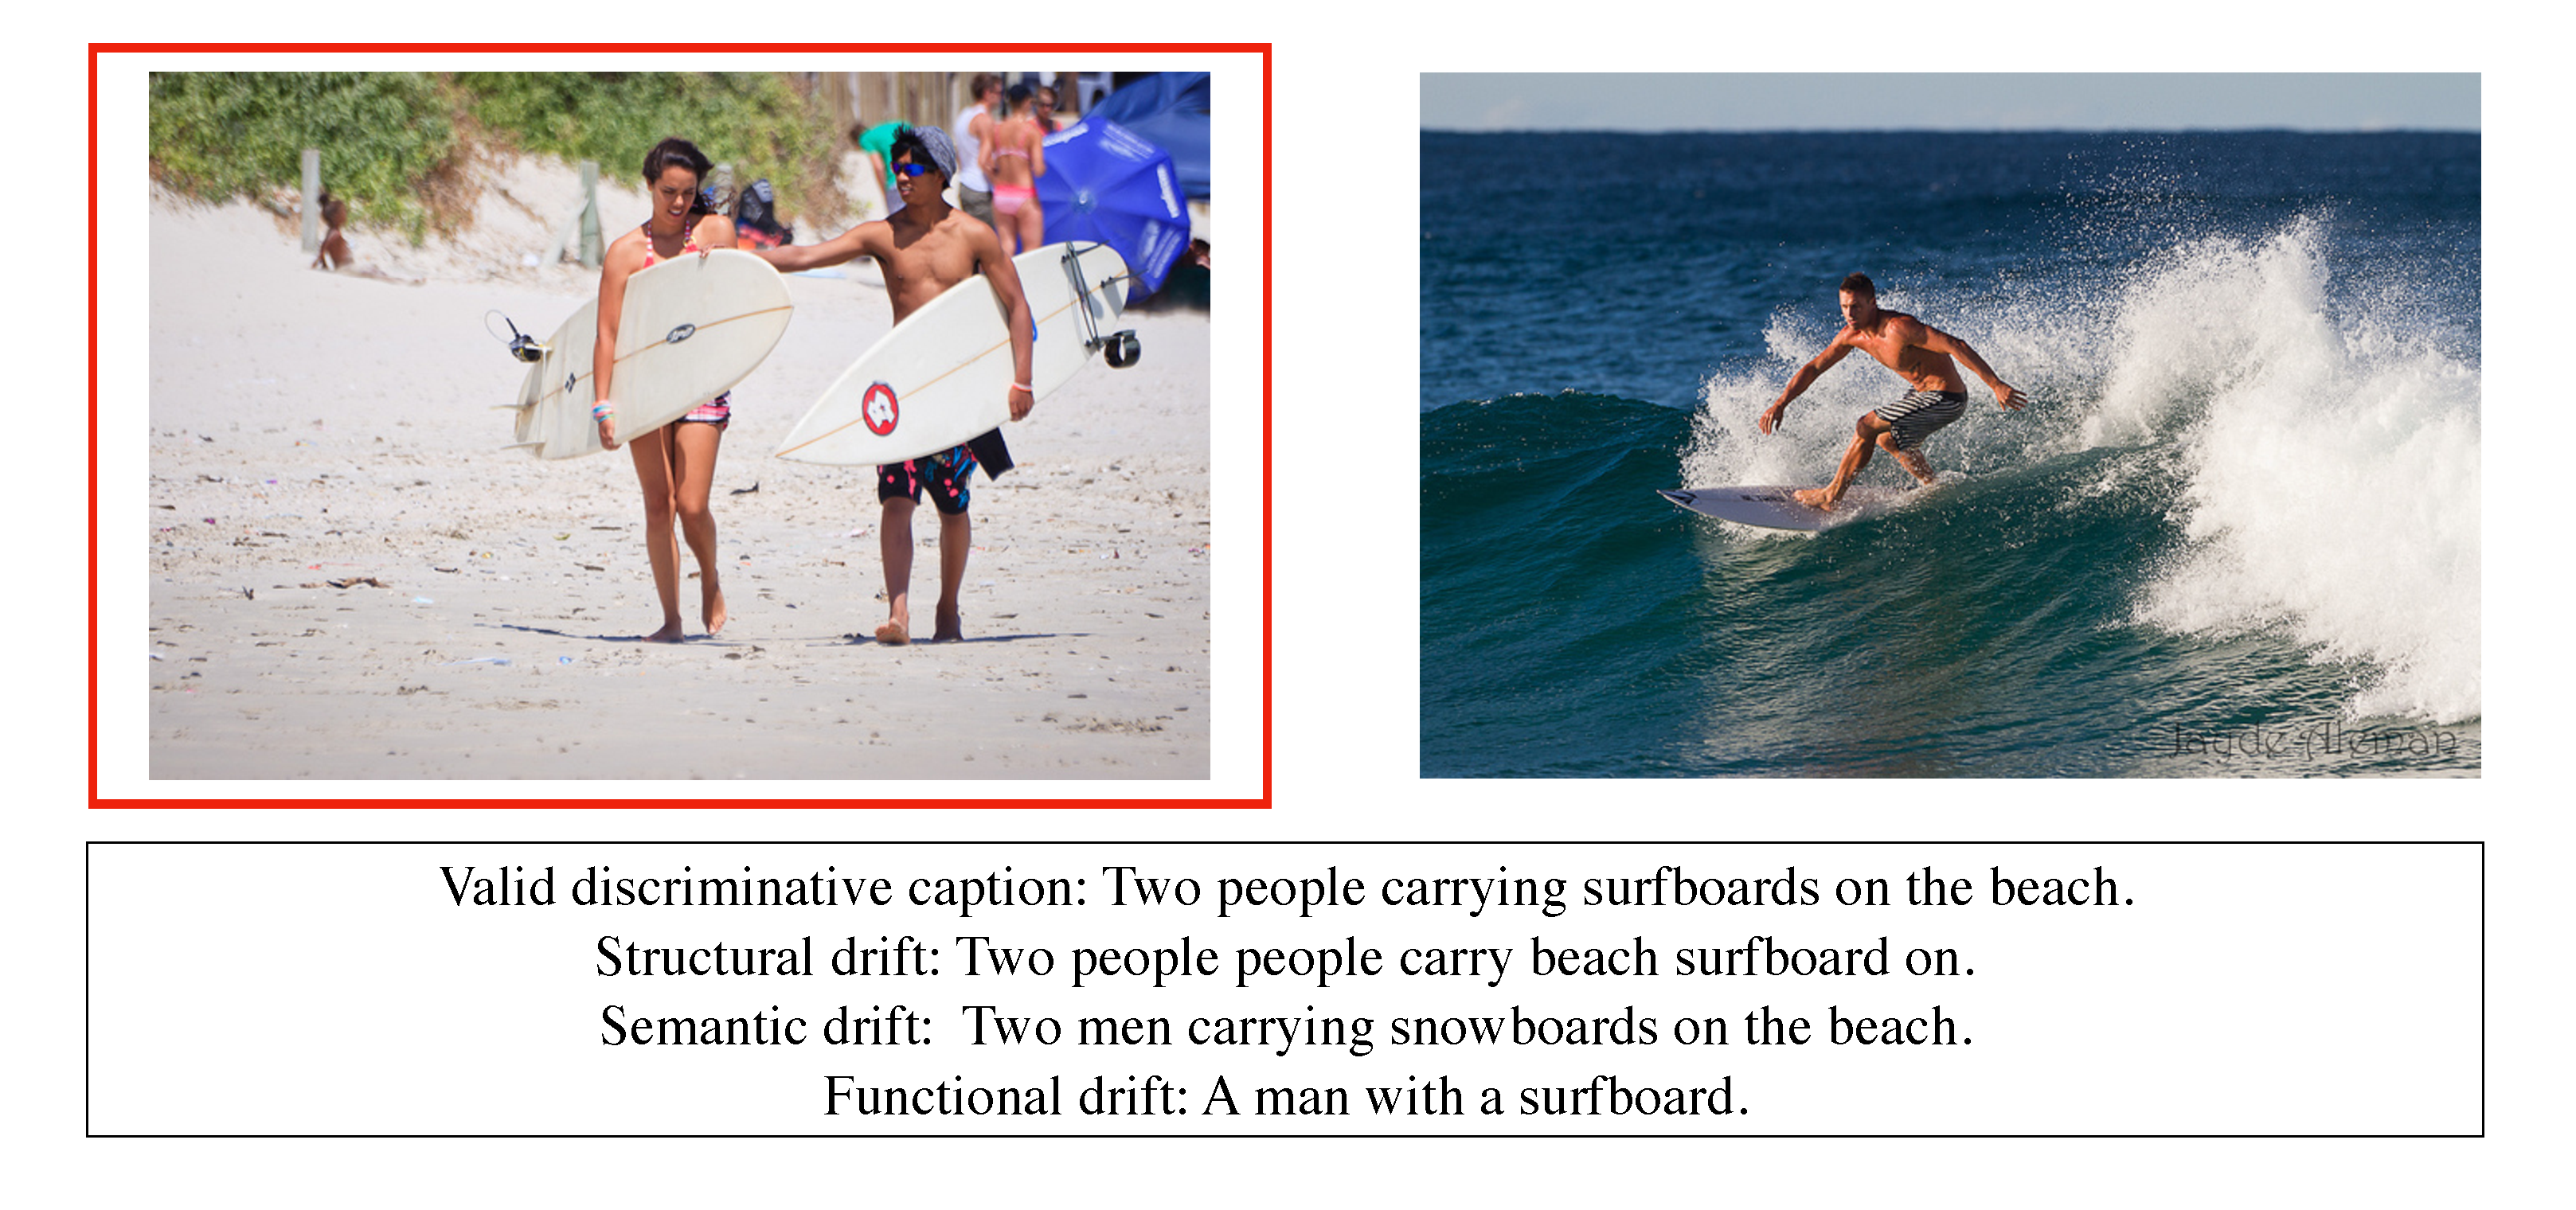
\includegraphics[width=0.9\linewidth]{images/COCO_drift_example_cropped.pdf}
	\caption{Example image pair. The target is marked by the red box.}
	\label{fig:coco_drift_example}
\end{figure}


\section{Measuring Language Drift}
\label{ld_metrics}

Some language drift metrics have been identified in the reviewed work. In particular, \cite{lazaridou2020multi} identified several measurements which are adopted in this thesis. These can be summarized as follows. 
\begin{itemize}
	\item \textit{Structural}, or, syntactic language drift can be measured as the log probability $P(m)$ of the generated message $m$ under a pre-trained unconditional language model. In this thesis, the pretrained Transformer XL model accessed through the \texttt{huggingface} library is used \parencite{dai2019transformer, wolf2019huggingface}.
	\item \textit{Semantic} language drift can be measured as the conditional log probability $P(m|i)$ of the generated message $m$ given the image $i$ under a pretrained image captioning model. In this thesis, the pretrained speaker models are used for this computation. %Another measure includes the $n$-gram overlap of generated messages and the ground-truth captions (ignoring stopwords) \cite{lazaridou2020multi}. Semantic drift is also addressed by \cite{lee2019countering}, \parencite{} but their approaches rather propose specific training methods than measures for identifying language drift, so their proposals wouldn't be considered here.
%	In alternative framings, semantic drift has been measured as the difference between the message semantics and the action taken by the receiver agent \cite{}. lu2020countering.
	\item Finally, \textit{pragmatic} language drift is assessed by \cite{lazaridou2020multi} as the discrepancy in referential success between human and listener agents in absense of structural or semantic drift. This is assessed by comparing the performance of humans to the performance of trained listener agents with a speaker trained to rerank the ground truth image captions (see above for details). 
\end{itemize}

However, given that the conducted experiments don't have access to human baseline data, pragamtic drift will have to be assessed differently. Although the proposed approach has the advantage of being task-agnostic, this work proposes to focus on a referential task drift approximating the pragmatic one. This approximation is referred to as \textit{functional} drift. Example messages which would exemplify all three kinds of language drift are presented in Figure \ref{fig:coco_drift_example}.

In this context, funtional drift refers to the deterioration of language which would make the referential task impossible for humans---for instance, leaving out critical content words. 
In contrast, other kinds of drift like structural drift might involve mixing up the word order, which nevertheless does not necessarily hinder the referential task, if distinctive content words are still present. For instance, the `functional drift' caption in Fig.~\ref{fig:coco_drift} would exemplify functional drift, while the caption ``A woman with a surfboard'' as well as the caption``With surfboard a a woman'' wouldn't, because they would mention a critical discriminative aspect. 
Crucially, the goal is to capture this drift in absense of human experiments. The difference between the proposed metric and pragmatic drift would be that functional drift is proposed in terms of the presense of discriminative words in the discription, which can be approximated as words or caption parts which have a higher probability for the target image than for the distractor. Thereby the metric becomes operationalizable under open-source pretrained models and does not depend on the availability of human data anymore. 

The following concrete operationalizations are tested in the experiments in order to capture functional drift. \begin{itemize}
	\item One approach for identifying functional language drift which is stable against compositional alternations within the caption and, therefore, isolates functional discriminativity, is the word overlap between the generated captions and the target vs. distractor ground truth captions, respectively. From a functional perspective, an optimal generated target caption maximizes the overlap with the target ground truth, while minimizing the overlap with the distractor ground truth. This idea is related to the omission score suggested by \cite{havrylov2017emergence} (also cf. \cite{andreas2016reasoning, gunel2020supervised}). This is also similar to the unigram metric employed by \cite{lazaridou2020multi}, but it adds the functional aspect via the difference computation. To sum up, the difference between the discrete word overlap of the target and generated captions and the overlap of the distractor and generated captions is computed. This is an intuitive step to take since ground truth captions are available for all images in the dataset. This metric is called \textit{discrete overlap} in the subsequent chapters.
	\item Complementarily, the idea described above is also formalized by computing the cosine similarity between the caption embeddings instead of word overlap scores. To this end, the trained speaker's embedding layer is used. This also hints at whether the trained embedding layer of the speaker, i.e., a representational layer, is affected by the functional learning signal. Again, the respective difference is computed as the drift metric and is expected to increase with successful task learning. This metric is called \textit{continuous overlap}.
	\item \pt{Depending on time constraints, this might be dropped altogether.} Finally, a rather exploratory approach is taken to measuring the recoverability of the target image based on the caption. Recoverability here is used in the loose sense of being able to reconstruct the intended image given the caption. Again, discriminative captions would present higher recoverability of the target comapred to the distractor. \pt{Either of two following approaches might be used, depending on what I might get to work} This is operationalized via a pretrained image-text retrieval model. Alternatively, this can be operationalized via a text-to-image model, where, ideally, the image produced from the generated caption would be more similar to the target than the distractor image. However, these metrics both heavily depend on the nature of the pretrained models as well as in the chosen image similarity metric. This metric is rather used in an exploratory way, in order to investigate if it alignes with intuitions and other metrics.
\end{itemize}
These metrics are used as diagnostic measures in order to identify potential sources of language drift. To this end, different experiments are conduceted. The section below outlines the hypothesized language drift behavior in the different experiments, as can be expected based on results from the literature.

\section{Hypotheses}
\label{hypos}

For simplicity of reference in the discussion of results, the different hypotheses are enumerated (note that these are rather research questions and not hypotheses in a strictly statistical sense). In this section, they are described on a conceptual level; more precise operationalizations in terms of presented experiments are described in \pt{FILL ME}.
First, hypotheses regarding language drift in the main experiments on the MS COCO dataset are described. 

As the speaker improves on the functional task, i.e., as the listener's accuracy increases and the functional loss is minimized, the following observations are hypothesized: \\
\newline 
% The speaker vocab size relation also to previous work 
\textbf{H1:} The structural drift is expected to increase. That is, the log probability of the generated captions under a pretrained model is expected to decrease. \newline
\textbf{H2:} The semantic drift is expected to increase. That is, the log probability of the generated caption given the target under the pretrained frozen speaker model is expected to decrease. \newline
\textbf{H3:} The discriminativity of the captions is expected to increase. That is, the word overlap difference is expected to increase, both for the discrete and the continuous overlap metrics. \newline
\textbf{H4:} Given that the pressure to stay close to the surface structure of natural language is provided by explicit structural constraints in the chosen model architecture (see Section \ref{architecture}), it is expected that both the structural and the semantic drifts increase as the weight of the structural constraints decreases, giving more room to functional learning. To investigate this, four reference games with different learning constraint parametrizations are conducted, ranging from no structural contraints to fully supervised structural learning. \newline
\textbf{H5:} The discriminativity of the captions is expected to increase less as the visual similarity of the target and the distractor increases. That is, the overlap metric values are expected to decrease, as the similarity of the distractors increases. This is expected due to the higher perceptual difficulty of discriminating images depicting similar things, and less potential for producing words that are true of the target, but not the distractor. Due to the intuitive necessity to produce more specific messages in order to refer to the target in presence of a highly similar distractor, it is also expected that the message length and possibly the specificity of the words increases. This will be analysed by investigating the produced parts of speech and message lengths, possibly accompanied by manual sample message inspection.\newline
\textbf{H6:}  The semantic and structural drifts are expected to be smaller in experiments where in the speaker is trained against a fixed (i.e., pretrained) listener compared to a listener trained jointly with the speaker. This is due to the observation made in prior work that especially semantic drift arises due to speaker-listener co-adaptation and the emergence of conventions among them. \newline
\textbf{H7*\footnote{The * indicated the optionality of this hypothesis based on available time}:} \pt{MS COCO vocab size variation to look at functional convergence speed, if there is time. It is more about the functional optimization potential than language drift though.} \newline
\textbf{H8*:} The recoverability of the target given the sampled caption is expected to increase with training. That is, the metric provided by the image-text retrieval model is expected to improve. \newline

In order to investigate the influence of the characteristics of the dataset on the drift, experiments with the manually annotated 3Dshapes dataset are conducted \parencite{burgess20183d}. Hypotheses \textbf{H1--H6} are also tested on 3Dshapes, but additional hypotheses about the comparison between MS COCO and 3Dshapes are explored. \\
\newline
\textbf{H9:} The relative strucutral drift is expected to be smaller compared to the MS COCO experiments. That is, the difference in the log probability of the message under the pretrained language model relative to the pretrained speaker is expected to be smaller than for MS COCO. This is expected due to the a priori given availability of exhasutively descriptive features in the training data. This availability is expected to alleviate the need of resorting to structurally misformed messages in order to adapt to the functional needs for the agents. \newline
%Message length, grammatical structure. 
%Granularity in random vs similar pairs.
%Again Ls, difference between joint and fixed listener.
\textbf{H10:} To deconfound the role of the availability of fully exhaustive descriptive captions and the size of the action space learned by the agent (which varies because MS COCO and 3Dshapes datasets are associated with vocabularies of different sizes) an experiment is conducted wherein the speaker is trained on both exhaustive and non-exhaustive captions. Comparing this experiment to the baseline 3Dshapes experiment on exhaustive captions only, following \textbf{H9}, higher structural drift is expected, as operationalized by lower caption log likelihoods of the messages under the pretrained LM.\newline

It is important to note that absolute values of the presented drift metrics should be interpreted with caution. Especially the structural drift metric is based on a model pretrained on possibly very different data distributions. Therefore, absolute log likelihood might be an artifact due to differences between the reference games data and pretraining data. Therefore, the metrics are intended to be interpreted comparatively within the training dynamics of the experiments, or between experiments with varying training configurations.

The next chapter finally turns to experiments in scope of which language drift using discussed metrics is investigated. 